While building software on a multitude of configurations, compilers, and platforms is CMake's greatest strength, it is also one of its greatest weaknesses as this often makes it hard for a programmer to figure out which build setups have actually been tested and are working for a given piece of software. Since version 3.19, CMake has a feature called presets that lets us handle these scenarios in a reliable and convenient way. Earlier, developers had to rely on documentation and fuzzy conventions to figure out the preferred configuration of a CMake project. Presets can specify the build directory, generators to use, target architecture, host toolchain, cache variables, and environment variables to use with a project. Since CMake 3.20, there are additional presets that affect the build and test phases as well.

For using presets, the top directory of a project must contain a file named either CMakePresets.json or CMakeUserPresets.json. If both files are present, they will be internally combined by parsing CMakePresets.json first and then  CMakeUserPresets.json. Both files have the same format but serve slightly different use cases:

\begin{itemize}
\item 
CMakePresets.json should be provided by the project itself and handle project-specific things, such as running CI builds or knowing which toolchains to use for cross-compilation if they are provided with the project itself. As CMakePresets.json is project-specific, it should not refer to any files or paths outside the project structure. Since these presets are tied in closely with the project, it is usually also kept under version control.

\item 
CMakeUserPresets.json, on the other hand, is usually defined by the developer for use on their own machine or build environment. CMakeUserPresets.json can be as specific as possible and contain paths outside the project or those that are unique to a particular system setup. As such, projects should not provide this file and also not put it under version control.
\end{itemize}

Presets are a great way of moving cache variables, compiler flags, and so on out of CMakeLists.txt files while still keeping the information available in a way that can be used with CMake and thus improve the portability of projects. If presets are available, they can be listed from the source directory by calling the following cmake -{}-listpresets, which will produce an output similar to this:

\begin{tcblisting}{commandshell={}}
Available configure presets:

  "ninja-debug" - Ninja (Debug)
  "ninja-release" - Ninja (Release)
\end{tcblisting}

This will list the name of the preset in quotes and the displayName property if set. To use properties from the command line, the name in quotes is used.

The CMake GUI will show all available presets in a source directory like this:

\begin{center}
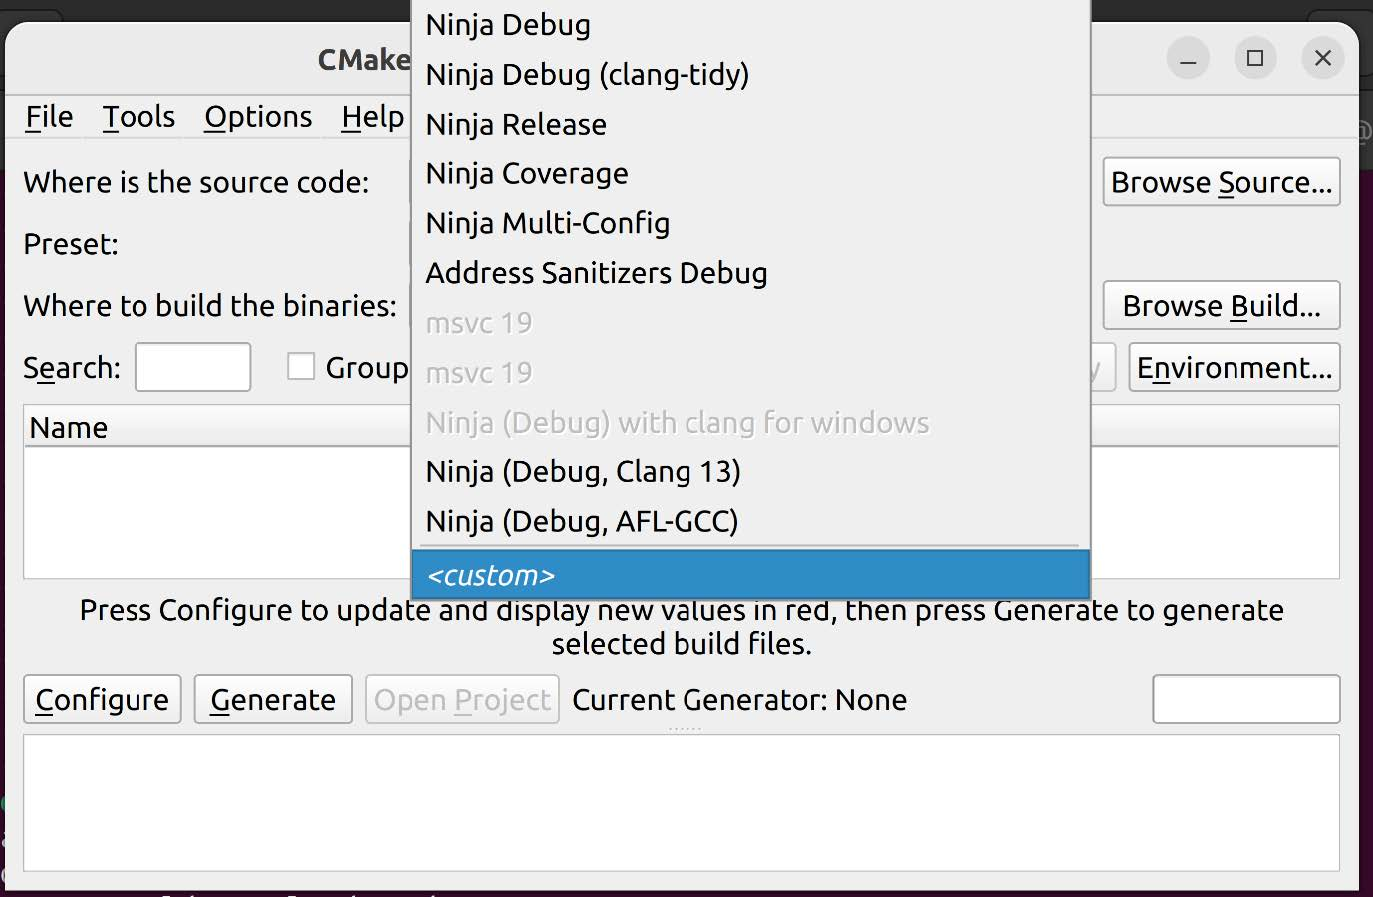
\includegraphics[width=0.8\textwidth]{content/2/chapter9/images/2.jpg}\\
Figure 9.1 – Listing available presets in the CMake GUI
\end{center}

As of version 3.21 of CMake, the ccmake command-line configuration tool does not support presets. Configure presets can be selected from the top-level directory by calling the following:

\begin{tcblisting}{commandshell={}}
cmake --preset=name
\end{tcblisting}

The overall structure of CMakePresets.json and CMakeUserPresets.json is like this:

\begin{lstlisting}[style=styleCMake]
{
	"version": 3,
	"cmakeMinimumRequired": {"major": 3,"minor": 21,"patch":
		0 },
	"configurePresets": [...],
	"buildPresets": [...],
	"testPresets": [...],
	"vendor": {
		"microsoft.com/VisualStudioSettings/CMake/1.9":
		{ "intelliSenseMode": "windows-msvc-x64"
	} }
}
\end{lstlisting}

The version field specifies the JSON schema to use. Version 1 is the first release from CMake 3.19 and only supports configurePresets. Version 2 adds buildPresets and testPresets and is available from CMake 3.20 and the version 3 adds more options and is available from CMake 3.21.

The optional cmakeMinimumRequired field may be used to define the minimum version of CMake needed to build this project. As the minimum requirement is usually also stated in the CMakeLists.txt files, this is often omitted.

The three lists, configurePresets, buildPresets, and testPresets, each contain a list of configurations for configuring, building, and testing the project. The presets for building and testing require the presence of at least one configuration preset, as we will see later in this section.

The vendor field contains an optional map of vendor- or IDE-specific information. CMake does not interpret the contents of this field except to verify the JSON format. The keys for the map should be the vendor-specific domain separated by slashes. In the previous example, the key for the vender presets is microsoft.com/VisualStudioSettings/CMake/1.9. The values inside the vendor fields can be of any valid JSON format.

To use presets, at least one configure preset that defines an environment for CMake to configure the build system has to be present. They should at least specify the build path and the generator to use when configuring. Often, a configure preset also sets common cache variables such as CMAKE\_BUILD\_TYPE for single-configuration generators. A preset containing a configure preset to build a project with the Ninja generator in debug mode might look like this:

\begin{lstlisting}[style=styleCMake]
{
	"version": 3,
	"configurePresets": [
	{
		"name": "ninja",
		"displayName": "Ninja Debug",
		"description": "build in debug mode using Ninja
		generator",
		"generator": "Ninja",
		"binaryDir": "build",
		"cacheVariables": { "CMAKE_BUILD_TYPE": "Debug" }
	}
	]
}
\end{lstlisting}

All presets must have a name that is unique within the preset block. As some GUI applications only show presets that have a displayName field assigned, setting this field is highly recommended.

\begin{tcolorbox}[colback=blue!5!white,colframe=blue!75!black,title=Naming Conventions for Presets]
It is good practice to name presets that are defined by the project in a
CMakePresets.json file in a way that they do not clash with names the developer might define in CMakeUserPresets.json. A common convention is to prefix project-defined presets with ci- to mark them as used by the CI environment.
\end{tcolorbox}

In versions 1 and 2 of the presets, the binaryDir and generator fields were mandatory; with version 3, they became optional. If either of the fields is not set, the behavior in this regard is the same as when CMake is used without presets. The command-line options for the CMake command will override the values specified in the presets where relevant. So, if binaryDir is set, it is automatically created when cmake -{}-preset= is called, although the value of it would be overridden if the -B option is passed to CMake.

Cache variables can either be defined as key:value pairs, as shown in the preceding example, or as a JSON object, which allows specifying the variable type. A file path could be specified like this:

\begin{lstlisting}[style=styleCMake]
"cacheVariables": {
	"CMAKE_TOOLCHAIN_FILE": {
		"type": "FILEPATH",
		"value": "${sourceDir}/cmake/toolchain.cmake"
	}
}
\end{lstlisting}

If used in the key:value form, the type is treated as STRING unless it is true or false (without quotes), in which case, it is interpreted as BOOL. Note \$\{sourceDir\} in the example, which is a macro that is expanded when the preset is used.

Here are a few well-known macros:

\begin{itemize}
\item 
\$\{sourceDir\}: This points to the project source directory and \$\{sourceParentDir\} points to the parent directory of the source directory. The directory name without the path of the source directory can be obtained with \$\{sourceDirName\}. For example, if \$\{sourceDir\} is /home/sandy/MyProject, \$\{sourceDirName\} would be MyProject and \$\{sourceParentDir\} would be /home/sandy/.

\item 
\$\{generator\}: This contains the generator as specified by the current preset used. For build and test presets, this contains the generator of the configure preset used.

\item 
\$\{hostSystemName\}: The system name of the host operating system, which is the same as the CMAKE\_HOST\_SYSTEM variable. The value is either the result of uname -s or Linux, Windows, or Darwin (for macOS).

\item
\$env\{<variable-name>\}: This contains the environment variable with the name <variable-name>. If the variable is defined in the preset with the environment field, this value is used instead of the value from the parent or system environment. Using \$penv\{<variable-name>\} works similarly, but the value is always taken from the parent environment and not from the environment field, even if it is defined. This allows prepending or appending values to existing environment variables. Appending or prepending variables is not possible with \$env\{...\} because it does not allow circular references. Note that while in a Windows environment, variables are case-insensitive; variables used in the presets are still case-sensitive. Because of this, it is recommended to keep the casing of environment variables consistent.

\item
\$vendor\{<macro-name>\}: This is an extension point for vendors of IDEs to
insert their own macros. Since CMake is not able to interpret these macros, presets
using \$vendor\{…\} macros will be ignored.

\item
\$\{dollar\}: This is a placeholder for the literal dollar sign, \$.
\end{itemize}

Modifying the environment for a preset works similarly to setting cache variables: by setting the environment field, which contains a map of key:value pairs. Environment variables are always set, even when the value is empty or null. Environment variables may reference each other as long as they do not contain circular references. Consider the following example:

\begin{lstlisting}[style=styleCMake]
{
	"version": 3,
	"configurePresets": [
	{
		"name": "ci-ninja",
		"generator": "Ninja",
		"binaryDir": "build",
		"environment": {
			"PATH": "${sourceDir}/scripts:$penv{PATH}",
			"LOCAL_PATH": "$env{PATH}",
			"EMPTY" : null
	}
	]
}
\end{lstlisting}

In this example, the PATH environment variable is modified by prepending a path from inside the project structure. Using the \$penv\{PATH\} macro ensures that the value is taken from outside the preset. The LOCAL\_PATH variable then references the modified PATH environment variable by using the \$env\{PATH\} macro. This reference is fine as long as the PATH environment variable does not contain \$env\{LOCAL\_PATH\}, which would create a circular reference. The EMPTY environment variable is unset by passing null. Note that null is not quoted. Unless a build preset or a test preset is used, the environment is not forwarded to the respective steps. If a build preset or a test preset is used, but the environment from the configure preset should not be applied, this can be explicitly stated when the inheritConfigureEnvironment field is set to false.

\subsubsubsection{9.2.1\hspace{0.2cm}继承预设}

Presets may inherit from other presets of the same type with the inherits field, which may contain either a single preset or a list of presets. When inheriting fields from the parent, a preset can be overridden or additional fields added. This is useful to avoid duplicating code for common building blocks. In combination with the hidden field, this can make a CMakePreset.json file smaller. Consider the following example:

\begin{lstlisting}[style=styleCMake]
{
	"version": 3,
	"configurePresets": [
	{
		"name": "ci-ninja",
		"generator": "Ninja",
		"hidden": true,
		"binaryDir": "build"
	},
	{
		"name": "ci-ninja-debug",
		"inherits": "ci-ninja",
		"cacheVariables": {
			"CMAKE_BUILD_TYPE": "Debug"
		}
	},
	{
		"name": "ci-ninja-release",
		"inherits": "ci-ninja",
		"cacheVariables": {
			"CMAKE_BUILD_TYPE": "Release"
		}
	}
	]
}
\end{lstlisting}

In the example, the ci-ninja-debug and ci-ninja-release presets both inherit from the hidden ci-ninja build preset and additionally set the CMAKE\_BUILD\_TYPE cache variable to the respective configuration. Hidden presets can still be used but will not show up when cmake -{}-list-presets is invoked. Presets defined in CMakeUserPreset.json may inherit from CMakePreset.json but not the other way around.

In the preceding example, the preset inherits from a single parent, but presets can also inherit from multiple parents. The following example shows how CMakeUserPreset. json working with CMakePreset.json from the previous example might look:

\begin{lstlisting}[style=styleCMake]
{
	"version": 3,
	"configurePresets": [
	{
		"name": "gcc-11",
		"hidden": true,
		"binaryDir": "build",
		"cacheVariables": {
			"CMAKE_C_COMPILER": "gcc-11",
			"CMAKE_CXX_COMPILER": "g++-11"
		}
	},
	{
		"name": "ninja-debug-gcc",
		"inherits": ["ci-ninja-debug","gcc-11"]
	},
	]
}
\end{lstlisting}

Here, the user supplies a preset that explicitly selects GCC 11 as a compiler named gcc-11. Later, the ninja-debug-gcc preset inherits the values from the ninja-debug preset that is defined in CMakePreset.json supplied by the project and combines it with the user-supplied gcc-11 preset. If two parent presets define different values for the same field, the value from the one first appearing in the inherits list takes precedence.

\subsubsubsection{9.2.2\hspace{0.2cm}预设的条件}

Sometimes presets only make sense under certain conditions, such as for a certain build platform. For instance, a configure preset that uses the Visual Studio generator would only be useful in a Windows environment. For these cases, presets can be disabled if the conditions are not met with the condition option. Any conditions defined in a parent preset are inherited. Conditions can be constants, string comparisons, or a check of whether a list contains a value. They are available from version 3 of the presets. The following configure preset would only be enabled if working on Windows:

\begin{lstlisting}[style=styleCMake]
{
	"name": "ci-msvc-19",
	"generator": "Visual Studio 16 2019",
	"binaryDir": "build",
	"condition": {
		"type": "equals",
		"lhs": "${hostSystemName}",
		"rhs": "Windows"
	}
}
\end{lstlisting}

In the preceding example, the build preset is enabled if the name of the host system is retrieved using the \$\{hostSystemName\} macro and then compared to the Windows string. If \$\{hostSystemName\} matches, then the preset is enabled, else it is disabled and trying to use it will result in an error. When comparing strings, casing matters: for case-insensitive tests, the matches or notMatches type, which takes a regex, could be used.

For more complex conditions, support nesting with Boolean logic with the allOf, anyOf, and not operators. For example, if a configure preset should only be enabled for Windows and Linux but not for macOS, the preset and the condition could look like this:

\begin{lstlisting}[style=styleCMake]
{
	"name": "WindowsAndLinuxOnly",
	"condition": {
		"type": "anyOf",
		"conditions": [
		{
			"type": "equals",
			"lhs": "${hostSystemName}",
			"rhs": "Windows"
		},
		{
			"type": "equals",
			"lhs": "${hostSystemName}",
			"rhs": "Linux"
		}
		]
	}
\end{lstlisting}

Each of the conditions could also contain further nested conditions if needed, although doing so will quickly increase the complexity of the presets.

So far, we have only seen configure presets in the examples, but as mentioned at the beginning of the chapter, there are also build presets and test presets. The syntax for build and test presets is very similar to configure presets and a lot of fields, such as name, displayName, and inherit, and conditions work the same as with configure presets.

Build presets have to specify a configure preset in the configurePreset field or inherit from another build preset that specifies the configure preset. The build directory is determined by the configure preset and the environment from the configure preset is inherited unless the inheritConfigureEnvironment field is set to false. Optionally, build presets can specify a list of targets to build. An example of a build preset could look like this:

\begin{lstlisting}[style=styleCMake]
{
	"version": 3,
	"configurePresets": [
	{
		"name": "ci-msvc-19",
		"displayName": "msvc 19",
		"description": "Configuring for msvc 19",
		"generator": "Visual Studio 16 2019",
		"binaryDir" : "build"
	}
	],
	"buildPresets": [
	{
		"name": "ci-msvc-debug",
		"configurePreset": "ci-msvc-19",
		"configuration": "Debug"
	},
	{
		"name": "ci-msvc-release",
		"configurePreset": "ci-msvc-19",
		"configuration": "Release"
	},
	{
		"name": "ci-documentation",
		"configurePreset": "ci-msvc-19",
		"targets": [
		"api-doc",
		"doc"
		]
	}
	]
}
\end{lstlisting}

In the preceding example, three build presets are defined. Two are used to specify the build configuration for Visual Studio and the third one lists the api-doc and doc targets as part of the documentation build. Invoking any of the ci-msvc build presets will build the "all" target, while ci-documentation will only build the listed targets. The list of available build presets can be retrieved with cmake -{}-build -{}-list-presets.

Test presets work very similar to build presets, except that they are used with CTest. Similarly, a call to ctest -{}-list-presets on the project root will list the available test presets. Test presets can be used to select or exclude certain tests, specify fixture options, or control the output of the tests. Most of the options for tests described in Chapter 7, Seamlessly Integrating Code Quality Tools with CMake, can be controlled from the test presets. An example of test presets could look like this:

\begin{lstlisting}[style=styleCMake]
{
	"version": 3,
	"configurePresets": [
	{
		"name": "ci-ninja",
		...
	}
	"testPresets": [
	{
		"name": "ci-feature-X",
		"configurePreset": "ci-ninja",
		"filter": {
			"include": {
				"name": "feature-X"
			},
			"exclude": {
				"label": "integration"
			}
		}
	}
	]
}
\end{lstlisting}

In the previous example, a test preset is added that filters the tests for any that include feature-X but excludes any tests that were labeled as integration. This is equivalent to invoking the following command from the build directory:

\begin{tcblisting}{commandshell={}}
ctest --tests-regex feature-X --label-exclude integration
\end{tcblisting}

CMake presets are arguably one of the few features that changed how CMake is used the most since the introduction of targets. They are a good compromise to deliver common configuration and build options together with the projects while still keeping the CMakeLists.txt file platform-agnostic. However, sometimes providing the necessary settings is not enough and you also want to share a build environment in which you are sure that the software compiles. One option to do this is by defining a build container that contains CMake and the necessary libraries.















